\chapter{EOM ps pulses and correlations}
In this chapter will be presented our study of an EOM based pulsed laser source to inspect the timing jitter.
\autoref{sec:Overview} will provide a comprehensive description of the experimental setup, to introduce a brief list of the jitter sources arising from the different components that will be located at \autoref{sec:Jitter Sources}.
We will then explain how the raw data are processed in \autoref{sec:DataAnalysis}, focusing in particular on \autoref{subsec:CentralPeakId} where the procedure behind the zero-delay peak recognition is explained.
Finally \autoref{EOMresults} presents the results we get from our analyses.


\section{Experimental setup overview}
\label{sec:Overview}
\begin{comment}

    These are the independently measured pulse lengths (FWHM), as function of the electrical bias imposed in the pulse compressor card.
    pulse_length[pulser_delay] = {-75.0: 22.332656690670724, -70.0: 33.28737362600773, -65.0: 34.562790842683, -60.0: 37.234513127783835, -55.0: 39.60844036795933, -50.0: 41.46464279128635, -45.0: 44.179758740180006, -40.0: 47.14183222708421, -35.0: 49.84367579880712, -30.0: 52.69148088494188, -25.0: 55.55398638871779, -20.0: 58.29172752901992, -15.0: 61.56981413564056, -10.0: 65.10148899764842, -5.0: 68.5853235124889, 0.0: 72.17479431215992, 5.0: 75.30042828585228, 10.0: 78.37782629223706, 15.0: 81.35991580449851}

    Queste misure sono state prese con un solo EOM, anche se l'autore riferisce che per pulse delays maggiori di -60 la lunghezza riportata qui corrisponde a quella che si osserverebbe nella configurazione con due EOM che invece utilizzo io nella mia tesi.
\end{comment}


For this first experimental chapter of this thesis we used a pulsed laser source originated by the use of electro-optic modulators (EOMs) on a starting CW laser source.
In \autoref{EOM_Setup_BIG} a zoomed out sketch of the experimental setup can be found. The image shows how the CW laser is coupled into a polarization-maintaining single-mode fiber (PM-SMF), and then electro-optically modulated by electronic signals shaped by a high-speed electronic circuit. All these components belong to the Orange shaded area of the picture.
On behalf of the electrical bias imposed in the PC interface, this part of the setup is responsible for the creation and the modulation of the optical pulses, according to an electronic delay imposed via PC.

The resulting pulsed laser source is then attenuated in intensity using a fiber splitter and then transferred with another fiber to the HBT setup, represented in \autoref{EOM_Setup_BIG} with a green colored area.
In this part of the setup the beam is equally divided with a fiber directional coupler, and then plugged into the second and third detectors of our SNSPD. As introduced in \autoref{sec:Def-Techniques}, the raw data, consisting of time-tagged detection events recorded by the ID1000 time tagger, will later be used to compute coincidences. These two final instruments consist in a "ID281" SNSPD together with a "ID1000" time tagger, both manifactured by ID Quantique SA.
For the specifications of the other components we remind to the article of the original designer of this setup, Mio Poortvliet \cite{MioArticle}.

\begin{figure}[hbtp]
\centering
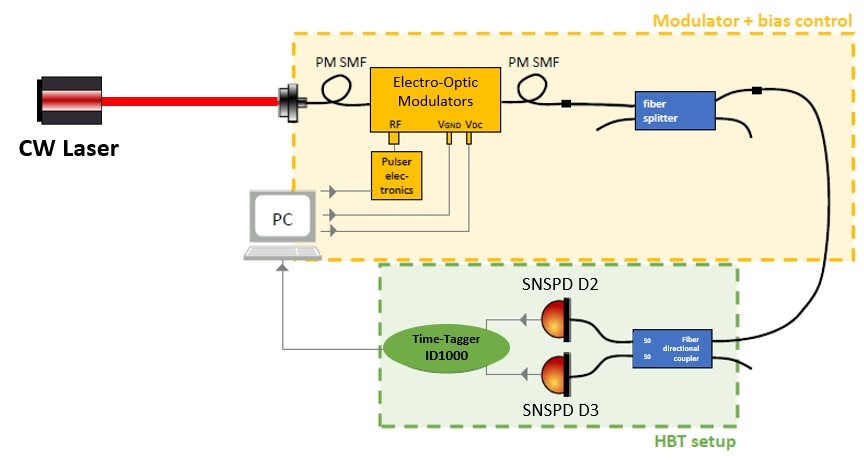
\includegraphics[width=1\textwidth]{EOMsetupBIG.jpg}
\caption{Schematic representation of the EOM based experimental setup}
\label{EOM_Setup_BIG}
\end{figure}
It is worth noting that in \autoref{EOM_Setup_BIG} the electro-optic modulation and the electronics that drives it, are only minimally shown. \autoref{EOM_PulseGen} provides a more detailed insight on what is actually driving the pulse generation.
The first three blocks from the top of the image represent the high speed electronics that generates the driving signal of the two EOMs.
At the very first stage, a field-programmable gate array (FPGA) generates a trigger signal in the form of a pulse pattern, that is passed to the pulse generator card. This system cam be operated in two regimes. For this project we specifically use the fast pulse generator, with a resolution of 1 ns and a configurable repetition rate ranging from 8 MHz to 500 MHz.
In our case the FPGA generates 1ns long pulses at the desired repetition rate of around 65MHz, corresponding to a repetition period of 15.2 ns.  
At this point, the signal is split and sent to two programmable delay lines with a resolution of 5 ps; a delay is applied to only one of the copies.
These two refined signals are combined with a 14-Gbps AND gate to obtain the customized pulse pattern whose width is adjustable based on the user-defined bias values for the programmable delay lines that we mentioned earlier.
Subsequently, the outputs of the pulse compressor board are the two pulse patterns resulting from a XOR port fed with the previous signal and a constant reference signal.

These two outputs, upon previous amplification, are then connected to the RF electrodes of the two cascaded EOMs, whose configuration is depicted in the lower part of \autoref{EOM_PulseGen}.  

\begin{figure}[hbtp]
\centering
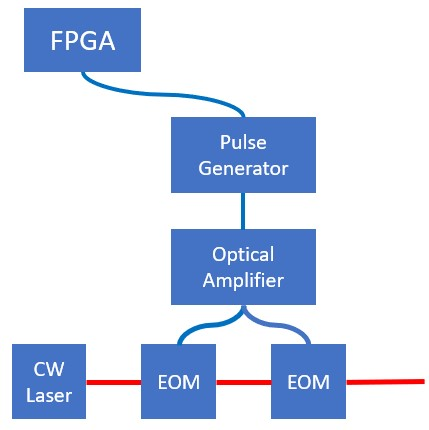
\includegraphics[width=0.4\textwidth]{EOM_Pulse_Sketch.jpg}
\caption{Schematic representation of the experimental tools involved into the pulse generation}
\label{EOM_PulseGen}
\end{figure}

\section{Relevant jitter in this experiment}
\label{sec:Jitter Sources}
After presenting the experimental architecture, this section examines the dominant sources of timing jitter introduced by the various components described above.
The pulser electronics encloses the first and main sources of timing jitter.
Referencing \autoref{EOM_PulseGen}, we identify within the FPGA, the first source of jitter, strictly followed by the effect of the several input discriminators implied in the architecture of the pulse generator card\cite{MioArticle}. The final purity affecting source, for this part comes from the ps-signal amplifier.
We assume that the electro-optic modulation of the CW laser is jitter-free, and that group velocity dispersion (GVD) only causes a slight temporal broadening of the pulses, without introducing significant distortions that could lead to timing jitter.
Focusing once again on \autoref{EOM_Setup_BIG}, it is worth noting that the time-tagged detection events collected from the ID1000 are also affected by other jitter contributions, at this point strictly related to the detection and processing routines in the two final instruments involved.
The single photon detector carries an intrinsic system-jitter contribution, and this is still an open research topic in the field of the SNSPDs \cite{SNSPD_Jit_1, SNSPD_Jit_2}.
Subsequently, as previously introduced, the electrical signals generated by the SNSPD are transferred to the time tagger. The ID1000 performs click identification based on a defined detection threshold; an improper choice of this threshold can cause delayed detections, introducing a deterministic source of jitter.
To the best of our knowledge, there may also be a contribution to timing jitter arising from internal clock drifts within the ID1000.

It is worth mentioning that, since we extensively use cables, we cannot exclude the possibility that electromagnetic noise—such as crosstalk—could introduce deterministic timing jitter at multiple points in the setup.

\section{Data analysis}
\label{sec:DataAnalysis}

\begin{figure}[hbtp]
\centering
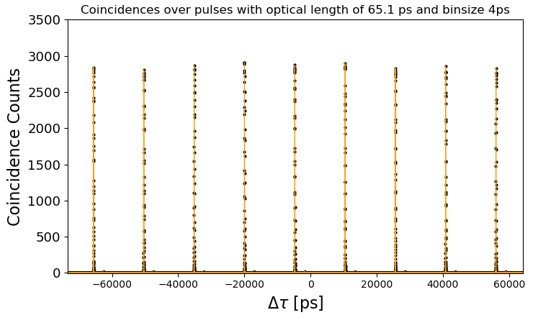
\includegraphics[width=1\textwidth]{CoincidenceExample.jpg}
\caption{Plot showing coincidence counts versus time, expressed in picoseconds. Image related to a measurement with a bias of -10 ps, correspoding to an independently measured duration of the pulse of 65.1 ps}
\label{CoincidenceCounts}
\end{figure}



\subsection{Data processing pipeline}
\label{subsec:Pipeline}
Ciaone

\begin{figure}[hbtp]
\centering
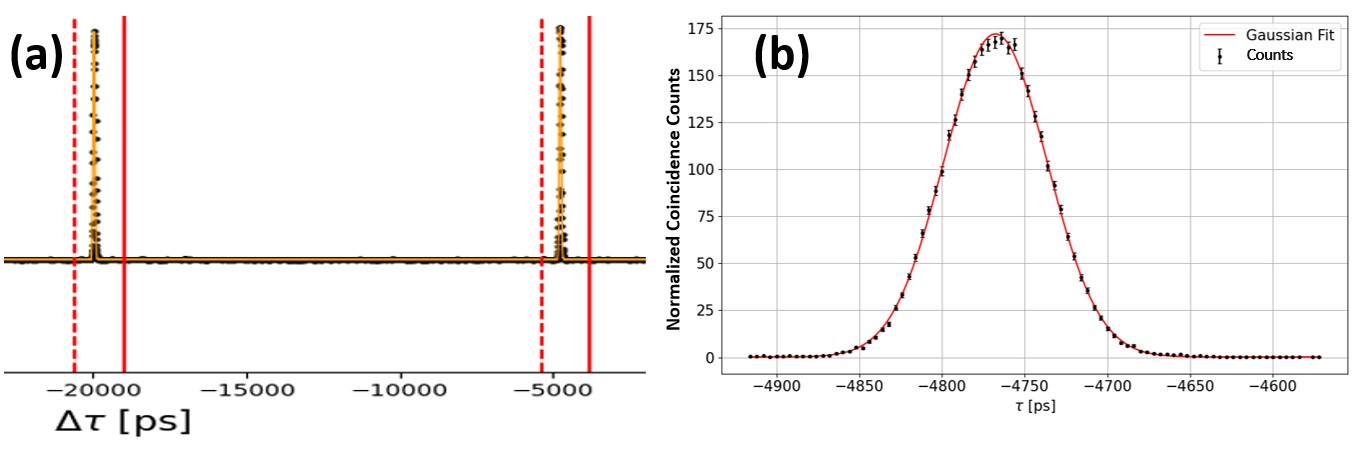
\includegraphics[width=1\textwidth]{NCountsFitting.jpg}
\caption{(a) Visual representation of the fitting intervals related to two different peaks. The red-dashed line represents the left boundary while the steady red one the right one. (b) Example of the gaussian fit obtained for one peak of the normalized counts plot.}
\label{FittingIMG}
\end{figure}


\subsection{Central peak identification}
\label{subsec:CentralPeakId}
Ciaone
\begin{figure}[hbtp]
\centering
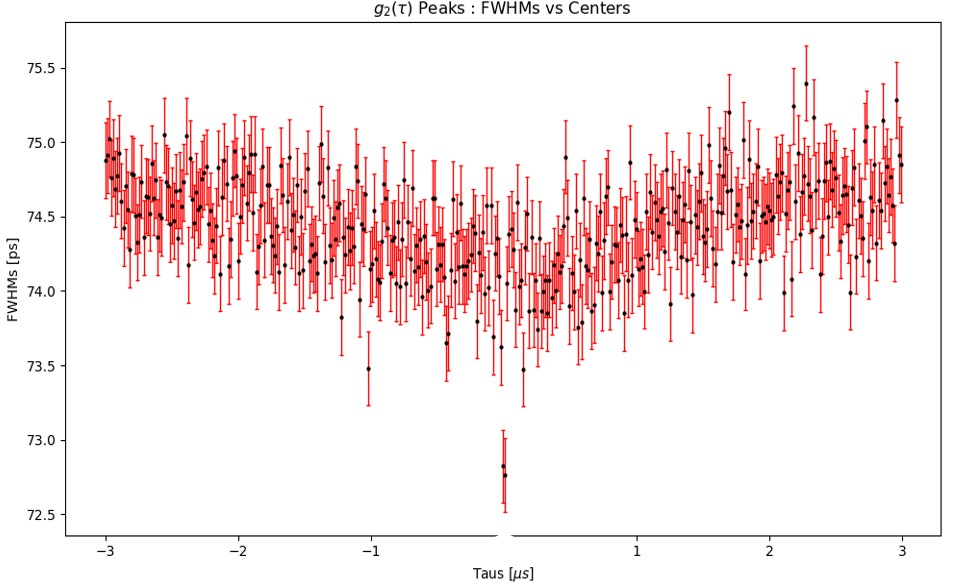
\includegraphics[width=1\textwidth]{FWHMvsTAU_Single.jpg}
\caption{PLot of FWHM vs tau coordinates of every peak fitted}
\label{FWHMvsTauSingle}
\end{figure}

\section{Results and Discussion}
\label{EOMresults}
ciaone

\begin{figure}[hbtp]
\centering
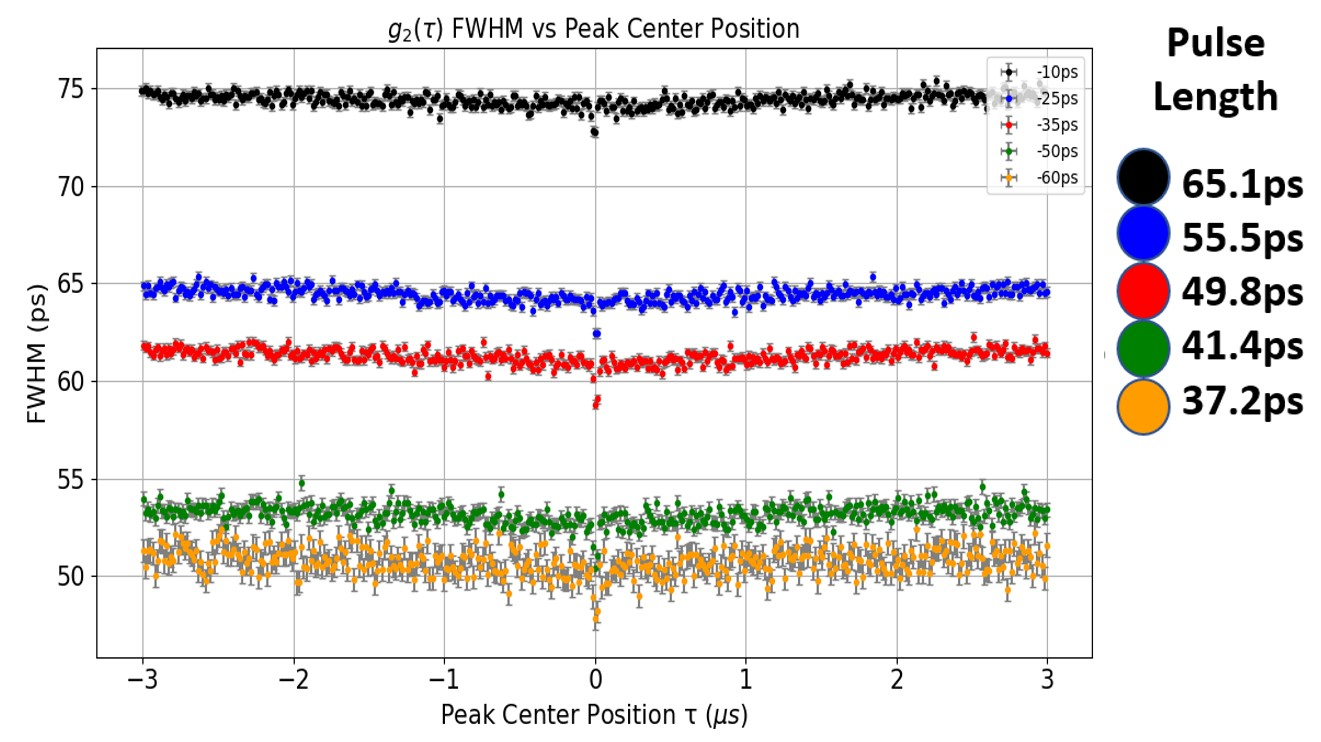
\includegraphics[width=1\textwidth]{FWHMvsTAU_ALL_Version2.jpg}
\caption{Ciaone}
\label{FWHMvsTauGeneral}
\end{figure}

\begin{figure}[hbtp]
\centering
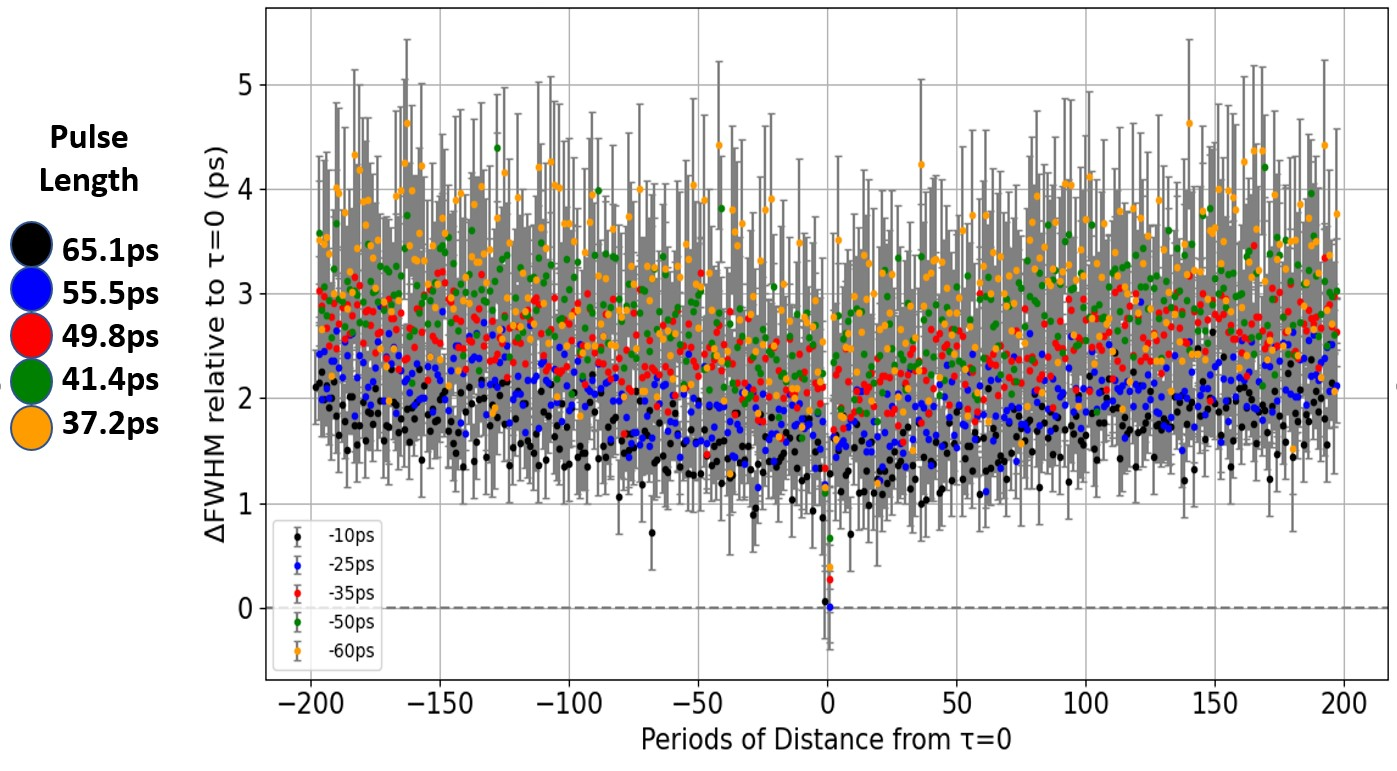
\includegraphics[width=1\textwidth]{DeltaFWHMvsPeriods.jpg}
\caption{Ciaone}
\label{DeltaFWHMvsPERIOD_General}
\end{figure}

\begin{figure}[hbtp]
\centering
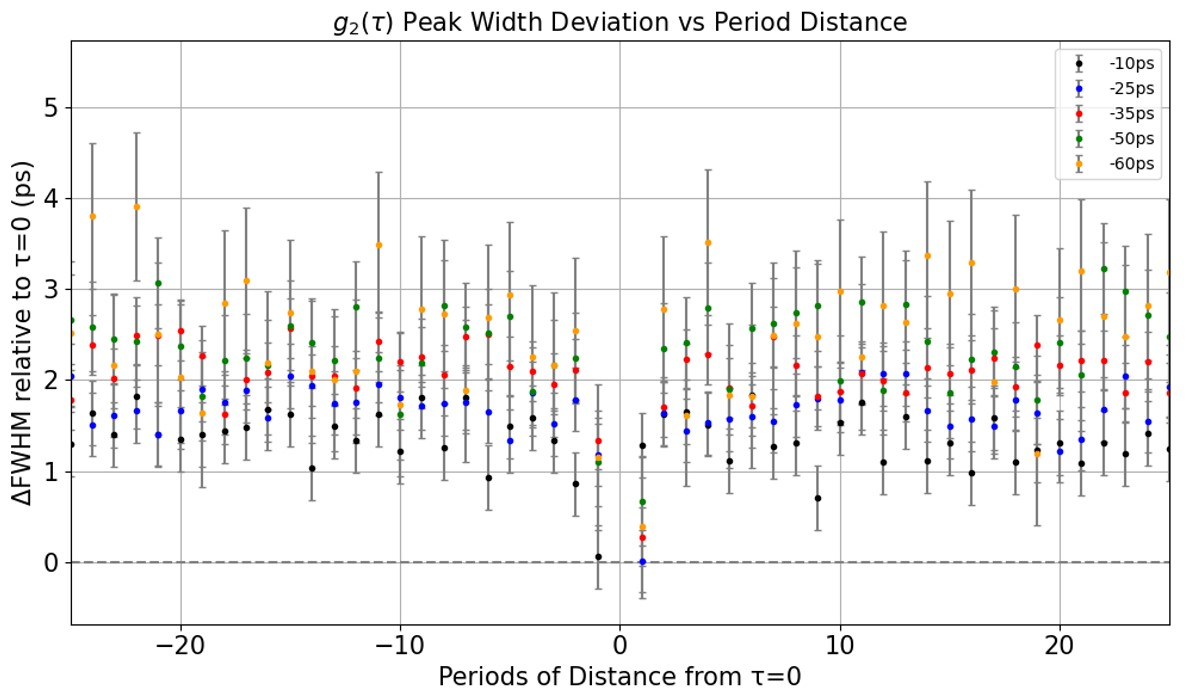
\includegraphics[width=1\textwidth]{DeltaFWHMvsPeriods_ZOOM.jpg}
\caption{Ciaone}
\label{DeltaFWHMvsPERIOD_ZOOM}
\end{figure}
